\documentclass{article}

% set font encoding for PDFLaTeX or XeLaTeX
\usepackage{graphicx}
\usepackage{ifxetex}
\usepackage{hyperref}

\ifxetex
  \usepackage{fontspec}
\else
  \usepackage[T1]{fontenc}
  \usepackage[utf8]{inputenc}
  \usepackage{lmodern}
\fi
\title{Actividad 1}
\author{Fisica Computacional 1\\
Corral Valdez Jesus Giovanni\\
Departamento de Física\\
Universidad de Sonora}
\date{}
% Enable SageTeX to run SageMath code right inside this LaTeX file.
% documentation: http://mirrors.ctan.org/macros/latex/contrib/sagetex/sagetexpackage.pdf
% \usepackage{sagetex}


\begin{document}
\maketitle
\section{Introducción}
La primera actividad consta de leer un capitulo del libro "Python for Data Analysis", de Wes McKinney\\
\begin{figure}[h]
  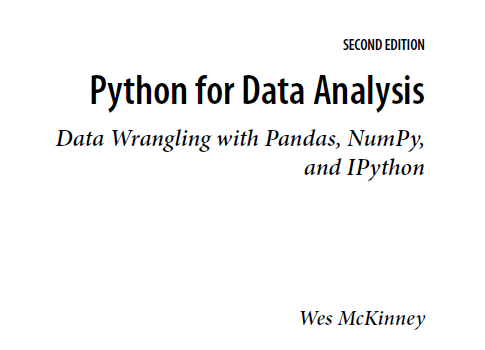
\includegraphics[width=\linewidth]{1-01.png}
\end{figure}
\clearpage

\section{Desarrollo}
Se leyó el capitulo 2\\
\begin{figure}[h]
  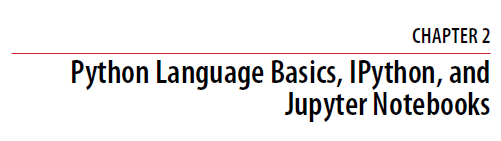
\includegraphics[width=\linewidth]{1-02.png}
\end{figure}
\clearpage
\begin{figure}[h]
  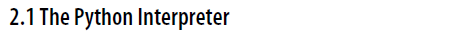
\includegraphics[width=\linewidth]{1-03.png}
\end{figure}
Python es un lenguaje interpretado que puede ejecutarse sencillamente desde su propio interpretador, pero quienes hacen análisis de datos prefieren hacer uso de intepretadores como IPython o Jupyter Notebook.\\

\begin{figure}[h]
  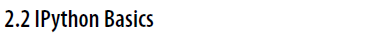
\includegraphics[width=\linewidth]{1-04.png}
\end{figure}
Uno de los mayores componentes del proyecto Jupyter es el "notebook", un tipo de documento interactivo para código, texto, visualizaciones de data y otras cosas. Este interact+ua con kernels.\\
En muchas plataformas Jupyter se abrira automaticamente en tu navegador web por default.\\
\begin{figure}[h]
  
\includegraphics[width=\linewidth]{1-05.png}
\end{figure}
\clearpage
Puedes crear un nuevo notebook y empezar a escribir en las celdas vacias. Al momento de salvarlo se creara un archivo con al extension .ipynb, el cual es un formato que contiene todo el contenido actual en el notebook. Estos pueden ser cargados y editados por otros usuarios de Jupyter\\
\begin{figure}[h]
  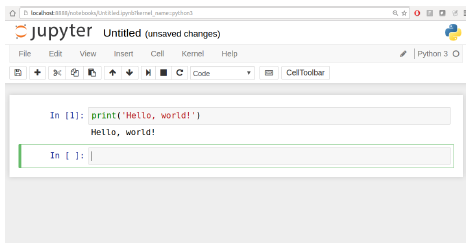
\includegraphics[width=\linewidth]{1-06.png}
\end{figure}
Uno de las mejores implementaciones de los editores de Python es la "Tab Completion", la cual al aplastar la tecla Tab durante estas escribiendo una expresion se te daran recomendaciones y opciones para terminar ese comando.\\
\begin{figure}[h]
  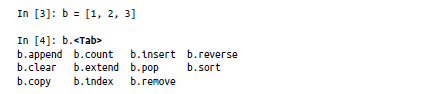
\includegraphics[width=\linewidth]{1-07.png}
\end{figure}
\clearpage
En Jupyter Notebook, es posible copiar y pegar codigo en cualquier celda de código y ejecutarlo. Otro dato útil es que conforme ha ido creciendo su popularidad y uso, se han creado cada vez mas "shortcuts" que nos facilitaran muchas acciones.\\
Una de las razones por la cual Jupyter es popular en analisis computacional es que se integra muy bien con la visualización y librerías de interfaz como matplotlib.
\begin{figure}[h]
  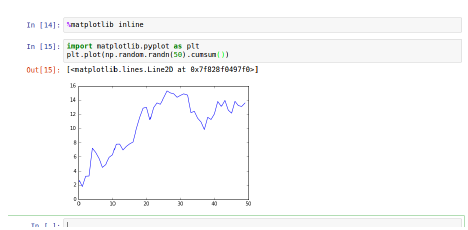
\includegraphics[width=\linewidth]{1-08.png}
\end{figure}
\begin{figure}[h]
  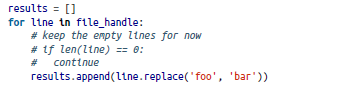
\includegraphics[width=\linewidth]{1-09.png}
\end{figure}
Esta sección nos hablar de conceptos esenciales del lenguaje de Python, el cual es distinguido por su enfásis en lectura, simplicidad y claridad.\\ Python utiliza espacios en blanco para estructurar el código, y en cambio los "punto y coma" son usados para separar múltiples sentencias pero es preferible no hacerlo ya que generalmente hace menos entendible el código.\\ Cada cosa en Python es considerado un "object" y tiene asociado un propio "type"(como string o function). Es posible hacer comentarios en el código que no afecten la ejecución de la celda, todo lo que se escriba precedido de un "hashtag":\\
\begin{figure}[h]
  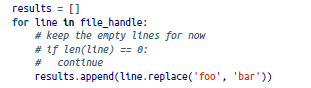
\includegraphics[width=\linewidth]{1-10.png}
\end{figure}
\clearpage
Puedes llamar funciones usando paréntesis, y casi cada objeto en Python tiene asociado funciones, conocidos como "métodos" los cuales tienen acceso a contenidos internos de estos objetos. Se llaman usando el siguiente código:\\
\begin{figure}[h]
  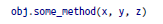
\includegraphics[width=\linewidth]{1-11.png}
\end{figure}
Cuando asignas una variable, se esta creando una referencia al objeto al lado derecho del signo de igual. Por ejemplo si escribimos "a = b", estamos haciendo que a y b sean el mismo objeto.\\
Las operaciones aritmeticas son muy parecidas a las que uno pensaría, las cuales son las siguientes:\\
\begin{figure}[h]
  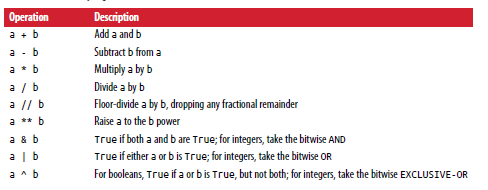
\includegraphics[width=\linewidth]{1-12.png}
\end{figure}
\clearpage

\section{Conclusiones}
Python es un lenguaje muy sencillo que la verdad no hace falta explicar casi cosas sobre el, tiene los clasicos "for, while, if", etc que tiene cualquier lenguaje, y los tipos númericos y de variables basicos. Ademas sus interpretadores como Jupyter Notebook hacen aun mas accesible el análisis de datos y la programación con este lenguaje.



\end{document}
